


\chapter{Sistema de controlo e monitorização}

\section{Design funcional}









\subsection{Requisitos funcionais}

\subsection{Requisitos não funcionais}







\section{Design técnico}



\subsection{Arquitetura do sistema}



\subsubsection{Camada de apresentação}


\subsubsection{Camada de negócio}



\subsubsection{Camada de dados}




\section{Diagrama de componentes}




\section{Sistema de interação}


\section{Descrição}


Modulos da daniela : Cc1110



\section{Arquitetura geral}

\begin{figure}[!htb]
	\centering
	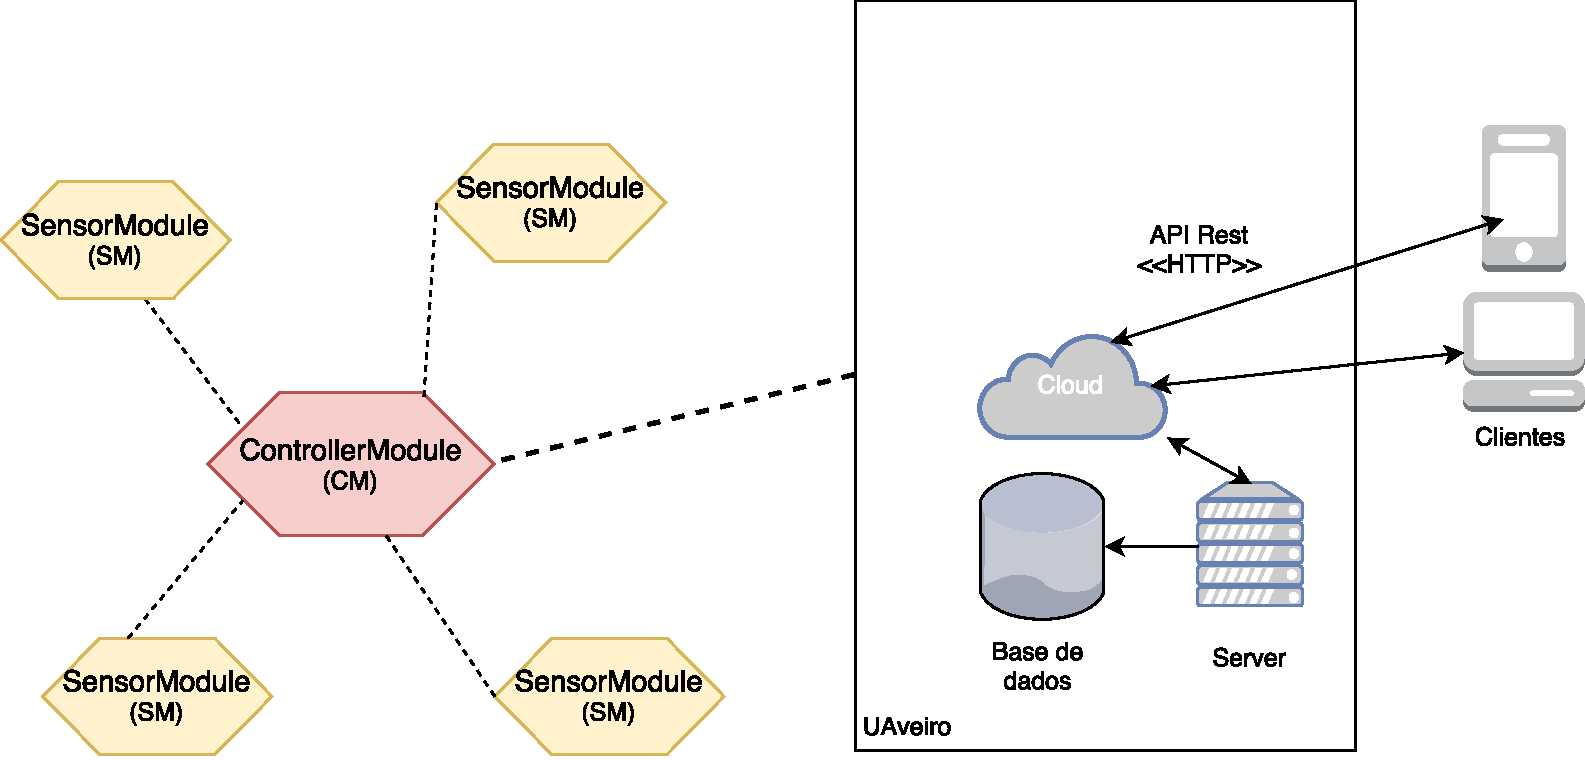
\includegraphics[scale=0.55]{esquemas/arquitetura_geral.pdf}
	\caption{Pirâmide do conhecimento: modelo DIKW}
	\label{dikw}
\end{figure}


\newpage


\section{Componentes}


\begin{figure}[!htb]
	\centering
	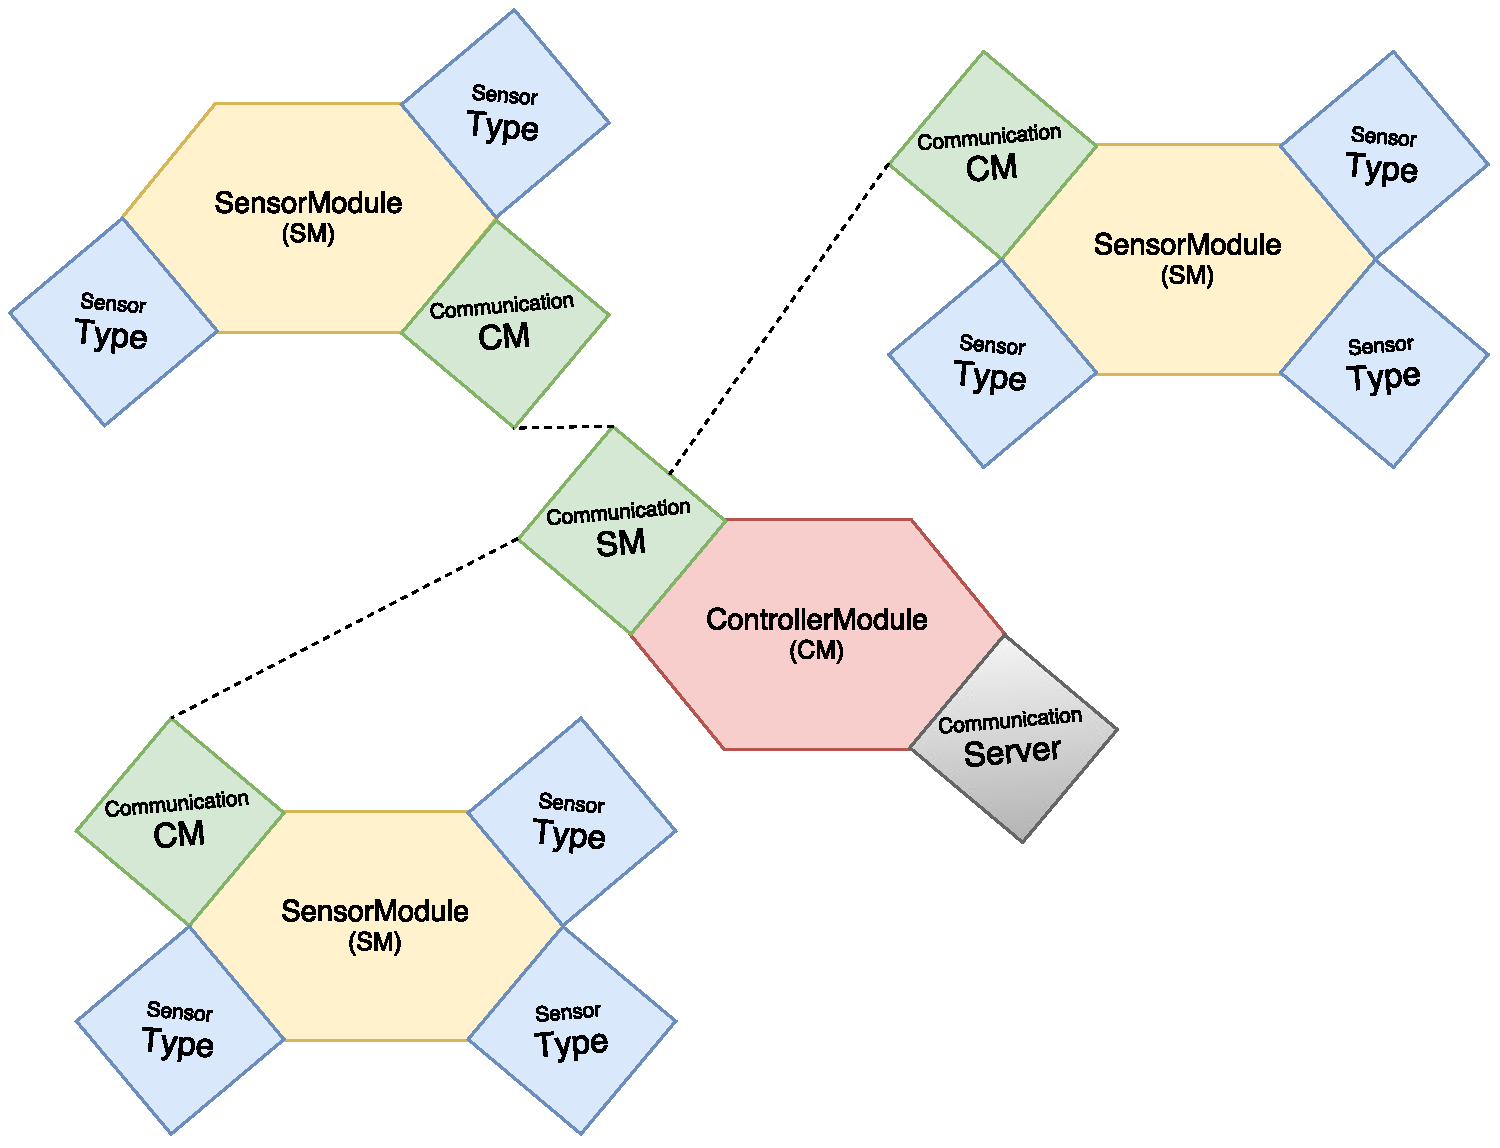
\includegraphics[scale=0.55]{esquemas/general-electronic-modules.pdf}
	\caption{Pirâmide do conhecimento: modelo DIKW}
	\label{dikw}
\end{figure}


\section{title}